\subsection{Kalibrierung} \label{kalibrierung-4}

\todo[inline]{Verantwortlich: Jonas}
Um die Präzision der vorhergesagten Emotionen weiter zu verbessern, wurde statt eines generellen Modells für alle Subjekte, der Ansatz eines personalisierten Modells geprüft. Dabei werden in einer kurzen Trainingsphase die Daten und Labels der Versuchsperson genutzt um das ML Modell zu trainieren, der Unterschied zum generalisieten Ansatz besteht hierbei, dass die charakteristischen Eigenschaften der Biosignale des Subjektes nicht über Vermischung mit denen der anderen Subjekte gemittelt werden, sondern zur Bestimmung des emotionalen Zustandes heran gezogen werden können. Die Gültigkeit des Modells beschränkt sich dabei auf die Testperson, für die das Modell gebildet wurde. Zur Validierung des Erfolges der Kalibrierung erfolgt nach der Trainingsphase eine Validierungsphase in der die Gültigkeit und die Präzision gemessen wird. \\

Zur Umsetzung wurde ein weiteres VR Emotionsinduktionsszenario erstellt. Hierbei werden in VR der Testperson auf einer virtuellen Leinwand 60 sekündige Videoausschnitte gezeigt und danach nach der Einschätzung des emotionalen Zustandes nach dem Circumplex Modell gefragt. Hierbei werden die gleichen Fragebögen wieder verwendet, die auch in der Hauptinduktion Verwendung finden (siehe. Abbildung \ref{fig:ablauf_kalibrierung}). Die Auswahl der Videos erfolgt dabei vor allem aus dem DEAP Datensatz (vgl. \cite{}). Dieser wurde insbesondere für die Validierungsphase mit weiteren Videosequenzen angereichert, deren Auswahl den gleichen Kriterien unterlag wie für den DEAP Datensatz. \\

Ausgewählt wurden für die beiden Kategorien Arousal und Valence jeweils drei Videos mit einem hohen und drei Videos mit einem niedrigen Wert. Insgesamt ergibt das für die Trainingsphase 12 Videos (3 Arousal hoch, 3 Arousal niedrig, 3 Valence hoch, 3 Valence niedrig). Diese Videos werden randomisiert hintereinander gezeigt. Damit ergibt sich eine Gesamtlaufzeit für ein Kalibrierungstraining von 15 bis 20 Minuten.  Nach dieser Zeit wartet der Proband, bis das ML Modell vollständig trainiert wurde, direkt in Anschluss daran werden ihm dann die 4 Validierungsvideos wieder randomisiert zwischen den vier Ausprägungen von Arousal und Valence gezeigt. Hierbei wird der emotionale Zustand des Probanden auch wieder nach jedem Video mit einem Fragebogen evaluiert. Anschließend erfolgt eine Auswertung mittels der Berechnung von Präzision und Recall des ML Modells. Diese Daten werden auch wieder innerhalb des Netzwerkes mittels UDP Paketen publiziert. \\
\begin{figure}[h]
    \centering
\begin{minipage}[t]{0.9\textwidth}
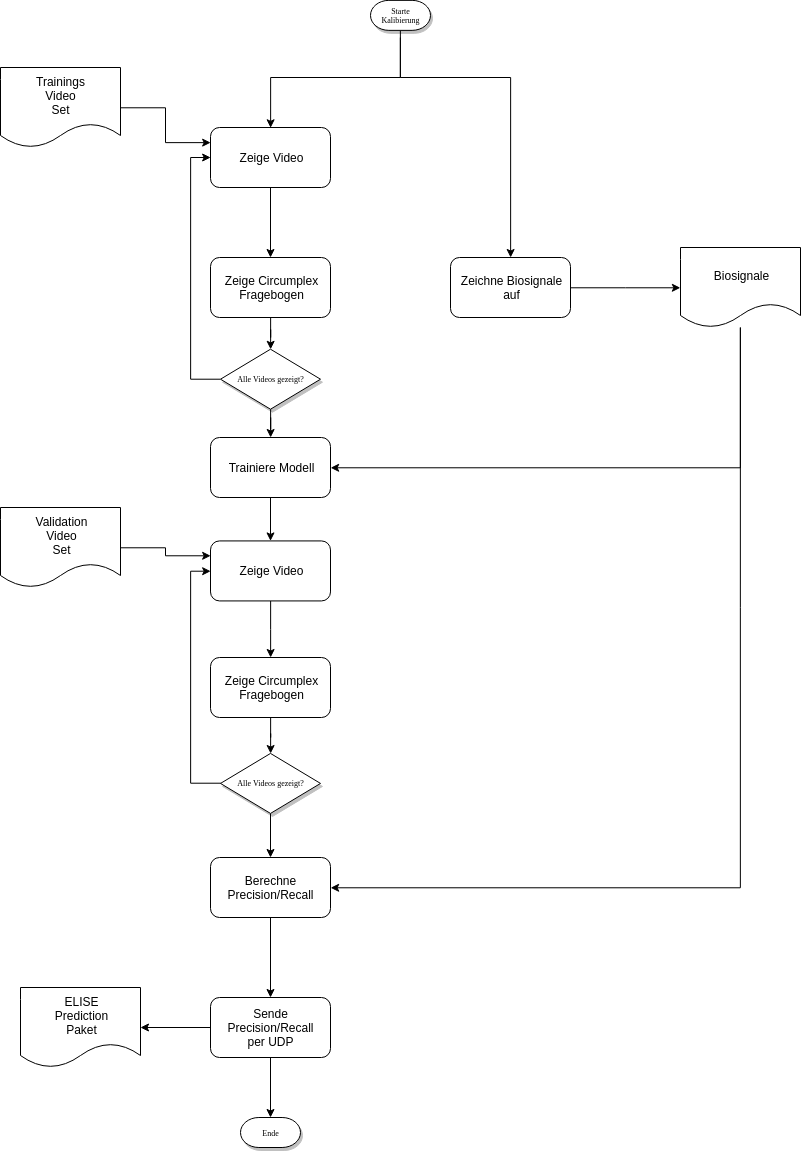
\includegraphics[width=\textwidth]{Images/kalibrierung_ablauf.png}
\end{minipage}
    \caption{Schematischer Ablauf der Kalibrierung}
    \label{fig:ablauf_kalibrierung}
\end{figure}





